%------------------------------------------------------
% Layouteinstellungen
%------------------------------------------------------
%-------------------------------------------------------
% Packages
%-------------------------------------------------------
\documentclass[a4paper, 11pt, twoside, numbers=noenddot, open=right, DIV=15, BCOR=1.3cm, listof=totocnumbered, bibliography=totocnumbered, appendixprefix=true, titlepage, headings=normal, parskip=relative]{scrbook}
\usepackage[ansinew]{inputenc}
\usepackage[T1]{fontenc}
\usepackage{mathptmx}
\linespread{1.1} 
\usepackage{floatflt} 
\usepackage{graphicx}
\usepackage[ngerman]{babel}
\usepackage{amsmath}
\usepackage{amssymb}
\usepackage[pdftex, bookmarks, bookmarksnumbered,pdfstartview=FitH]{hyperref}
\usepackage{colortbl}
\usepackage{float} 		
\usepackage{microtype}
\usepackage{sidecap}
\usepackage{cite}
\usepackage[numbers]{natbib}
\usepackage{picins}
\usepackage{dirtree}
\usepackage{wrapfig}
\usepackage{tabularx}
\usepackage{multirow}
\usepackage{multicol}
\usepackage{pdfpages}
\usepackage{enumitem}
\usepackage{trfsigns}
\usepackage{everysel}
\usepackage{subfig}
%\usepackage[plainpages=false, pdfpagelabels]{hyperref}

%-------------------------------------------------------
% Packete um Inkscape Schriften durch latex zu substituieren
%-------------------------------------------------------

\usepackage{import}
\graphicspath{{images/}} % Hier steht Pfad zu den Grafiken

%-------------------------------------------------------
% Darstellung �berschrift mit Serifen und Kapitel einrahmen
%-------------------------------------------------------
%\setkomafont{sectioning}{\bfseries}
\setkomafont{sectioning}{\slshape\bfseries}
%\renewcommand{\familydefault}{\sfdefault}
%\setkomafont{sectioning}{\bfseries}

%\renewcommand*{\chapterheadstartvskip}{\vspace*{-40pt}}

%\newcommand*{\ORIGchapterheadstartvskip}{}%
%\let\ORIGchapterheadstartvskip=\chapterheadstartvskip
%\renewcommand*{\chapterheadstartvskip}{%
%  \ORIGchapterheadstartvskip
%  {%
%    \setlength{\parskip}{0pt}%
%    \noindent\rule[-0.1\baselineskip]{\linewidth}{0.8pt}\par
%  }%
%}
\newcommand*{\ORIGchapterheadendvskip}{}%
\let\ORIGchapterheadendvskip=\chapterheadendvskip
\renewcommand*{\chapterheadendvskip}{%
  {%
    \setlength{\parskip}{0pt}%
    \noindent\rule[0.5\baselineskip]{\linewidth}{0.5pt}\par
  }%
  \ORIGchapterheadendvskip
}

%-------------------------------------------------------
% Matlab Code einbinden
%-------------------------------------------------------

\usepackage{listings}
\usepackage{color}
\usepackage[svgnames]{xcolor} 
\lstset{
   language = Matlab,
   basicstyle = {\ttfamily\scriptsize},
   keywordstyle = \color{black!80!black!100},
   identifierstyle = ,
   commentstyle = \color{black!50!black!100},
   stringstyle = \ttfamily,
   breaklines = true,
   numbers = left,
   numberstyle = \scriptsize,
   frame = single,
   backgroundcolor = \color{white!3}
}

%-------------------------------------------------------
% Zus�tzliches Layout Rand oben
%-------------------------------------------------------

\setlength{\topmargin}{-1.2 cm}      	  

%-------------------------------------------------------
%Absatzeinzug
%-------------------------------------------------------

\setparsizes{0pt}{4pt}{0pt plus 1fill}
%\setparsizes{0pt}{2pt}{0pt plus 1fill} 

%-------------------------------------------------------
% Kopf- und Fusszeile
%-------------------------------------------------------

\usepackage[automark]{scrpage2}
\pagestyle{scrheadings}

\clearscrheadfoot
\ohead{\headmark}
\ofoot[\pagemark]{\pagemark}
\setheadsepline{0.5pt}
%\setfootsepline{0.5pt}

%-------------------------------------------------------
% Tabellen Schattierung
%-------------------------------------------------------

\definecolor{Blue}{rgb}{0.0667,0.4000,0.6784}
\definecolor{Gray}{rgb}{0.9,0.9,0.9}

%-------------------------------------------------------
% Darstellung Formeln etc.
%-------------------------------------------------------

% F�r Matrizen und Vektoren
\newcommand{\m}[1]{\underline{#1}}
\newcommand{\mh}[1]{\underline{\hat{#1}}}
\newcommand{\mt}[1]{\underline{\tilde{#1}}}
\newcommand{\mb}[1]{\underline{\bar{#1}}}
\newcommand{\mhb}[1]{\underline{\hat{\bar{#1}}}}
\newcommand{\lt}[1]{\left\|{#1}\right\|_{2}}
\newcommand{\lm}[1]{\left\|{#1}\right\|_{\infty}}
\newcommand{\mr}[1]{#1}
\newcommand{\eq}[1]{\begin{align}{#1}\end{align}}
\newcommand{\seq}[1]{\begin{subequations}\begin{align}{#1}\end{align}\end{subequations}}

\definecolor{mainc}{RGB}{0,100,166} % Main Color ZHAW
\definecolor{subsc}{RGB}{206,0,60} % Subsidiary color School of Engineering
\definecolor{greyp}{RGB}{154,154,156} % Grey (pale)
\definecolor{greyd}{RGB}{74,93,104} % Alternate grey (dark)
\definecolor{grayd}{RGB}{100,100,100} % Alternate grey (dark)

% Color definitions for text and math mode for easy use
\newcommand{\tmc}[1]{\textcolor{mainc}{#1}}
\newcommand{\tsc}[1]{\textcolor{subsc}{#1}}
\newcommand{\tgd}[1]{\textcolor{greyd}{#1}}

\newcommand{\mmc}[1]{{\color{mainc} #1}}
\newcommand{\msc}[1]{{\color{subsc} #1}}
\newcommand{\mgd}[1]{{\color{greyd} #1}}




%------------------------------------------------------
\begin{document}
%------------------------------------------------------
% Importiere Titelseite
%------------------------------------------------------
%------------------------------------------------------------
\begin{titlepage}
%------------------------------------------------------------
	\vspace*{0cm}
%------------------------------------------------------------
\begin{flushright}

\includegraphics[width=4cm]{images/logo-zhaw.pdf}
\end{flushright}
\begin{center}
		\vspace{1.5cm}
  	\begin{center}
    	\Large{Projektarbeit}
    \end{center}
		\vspace{0.5cm}
				\huge{\bfseries{Theorem der endlos tippenden Affen}}
		\vspace{0.5cm}
  	\begin{center}
      \Large{Institut f�r Irgendwas}
    \end{center}
		\vspace{2cm}
		\large
		{
			\begin{tabular}{lll}
			  Ausgabe:	&	01. November 2049\\
				Einreichung: & 13. Mai 2050\\\\
				Autoren:          & Max Muster\\
				 & Moritz Muster\\
				Betreuer:				&	Prof. Dr. Max Muster\\
				Industriepartner: & Max Muster, Irgendwas AG \\
				Externer Experte: & Dr. Max Muster
			\end{tabular}
		}
\end{center}
		
%------------------------------------------------------------
\end{titlepage}
%------------------------------------------------------------

%------------------------------------------------------
% Erstelle Inhaltsverzeichnis und Zusammenfassung
%------------------------------------------------------
\frontmatter
\chapter*{Zusammenfassung}

Gegenstand der vorliegenden Arbeit ist...



\cleardoublepage

\includepdf[pages=-, pagecommand={\thispagestyle{scrplain} \begin{flushright}
\includegraphics[width=3cm,keepaspectratio]{images/logo-zhaw.pdf}
\end{flushright}}, noautoscale=true, offset=0.0cm -1.5cm,width=1.0\textwidth]{images/Erklaerung_PA.pdf}
\setcounter{tocdepth}{1} % F�hre im Inhaltsverzeichnis nur Titel und Untertitel auf
\tableofcontents
\chapter*{Abk\"urzungen}
\label{sec:begriffserklaerung}

\begin{table}[H]
\begin{tabular}{p{0.30\textwidth}l}
\bfseries\itshape{OMG} & Oh my God!\\
\end{tabular}
\end{table}

%------------------------------------------------------
% Importiere Einzeldokumente
%------------------------------------------------------
\mainmatter
\chapter{Ich bin ein Kapitel}
\label{sec:regelung}

%----------------------------------------------------------------------------------------------
\section{Ich bin ein Titel}
\label{sec:ichbineintitel}
%----------------------------------------------------------------------------------------------

Dumm ist der der dummes tut. Dumm ist der der dummes tut. Dumm ist der der dummes tut. Dumm ist der der dummes tut. Dumm ist der der dummes tut. Dumm ist der der dummes tut. Dumm ist der der dummes tut. Dumm ist der der dummes tut. Dumm ist der der dummes tut.\\ % \\ --> Neue Zeile
Dumm ist der der dummes tut. Dumm ist der der dummes tut. Dumm ist der der dummes tut. Dumm ist der der dummes tut. Dumm ist der der dummes tut. Dumm ist der der dummes tut. Dumm ist der der dummes tut. Dumm ist der der dummes tut. Dumm ist der der dummes tut.
% Abstand --> Neuer Absatz

Dumm ist der der dummes tut. Dumm ist der der dummes tut. Dumm ist der der dummes tut. Dumm ist der der dummes tut. Dumm ist der der dummes tut. Dumm ist der der dummes tut. Dumm ist der der dummes tut. Dumm ist der der dummes tut. Dumm ist der der dummes tut.

\subsection{Ich bin ein Untertitel}

Dumm ist der der dummes tut. Dumm ist der der dummes tut. Dumm ist der der dummes tut. Dumm ist der der dummes tut. Dumm ist der der dummes tut. Dumm ist der der dummes tut. Dumm ist der der dummes tut. Dumm ist der der dummes tut. Dumm ist der der dummes tut. 

\subsubsection{Ich bin ein Unter-Untertitel}

Dumm ist der der dummes tut. Dumm ist der der dummes tut. Dumm ist der der dummes tut. Dumm ist der der dummes tut. Dumm ist der der dummes tut. Dumm ist der der dummes tut. Dumm ist der der dummes tut. Dumm ist der der dummes tut. Dumm ist der der dummes tut. 

\minisec{Ich bin ein Unter-Untertitel mit wenig Abstand bis zum Text}

Dumm ist der der dummes tut. Dumm ist der der dummes tut. Dumm ist der der dummes tut. Dumm ist der der dummes tut. Dumm ist der der dummes tut. Dumm ist der der dummes tut. Dumm ist der der dummes tut. Dumm ist der der dummes tut. Dumm ist der der dummes tut. 

\newpage % -> Begine auf einer neuen Seite
%----------------------------------------------------------------------------------------------
\section{Einige Gleichungen}
%----------------------------------------------------------------------------------------------

\subsection{Eine Gleichung}

\eq{
	y = f\left(x\right)
}

\subsection{Eine Gleichungsfolge mit Text}

% Befehl von pmic \seq
\seq{
 	u &= R_1i_1 + L_1\frac{d}{dt}i_1 -M\frac{d}{dt}i_2 + k_{m1}\frac{d}{dt}x & \mbox{(Spule bzw. Spulenpaar)} \label{eq:voice_coil_dynamik_a}\\
 	0 &= R_2i_2 + L_2\frac{d}{dt}i_2 -M\frac{d}{dt}i_1 + k_{m2}\frac{d}{dt}x & \mbox{(Kurzschlussring)}\\
 	m\frac{d^2}{dt^2}x &= w_{e1}i_1 + w_{e2}i_2 & \mbox{(Mechanik)}
	\label{eq:voice_coil_dynamik_c}
}

\subsection{Matrizen}

\minisec{Zwei Matrizen}

\begin{align}
\mh{A}_{ds} &= 
	\left[
		\begin{array}{rrrrrr}
    0.8565  &  0.0218  &  0.0211  & -0.0096  & -0.0050  &  0.0080 \\
    0.0156  &  0.8659  &  0.0222  &  0.0019  &  0.0226  &  0.0124 \\
    0.0154  &  0.0204  &  0.8655  &  0.0034  & -0.0070  & -0.0080 \\
   -0.0003  & -0.0041  &  0.0042  &  0.9444  &  0.0051  &  0.0039 \\
    0.0043  & -0.0018  & -0.0037  &  0.0062  &  0.9452  &  0.0066 \\
   -0.0040  &  0.0034  &  0.0004  &  0.0034  &  0.0058  &  0.9447
		\end{array}
	\right] \notag \\
	\mh{B}_{ds} &= 
	\left[
		\begin{array}{rrrrrr}
   23.6438  & -4.1978  & -4.5305  & -1.0673  & -0.6754  &  2.8364 \\
    1.5117  & 20.5480  & -4.9742  &  0.5737  &  4.3086  &  1.1824 \\
   -3.5779  & -2.1936  & 21.4407  & -0.4329  &  0.6942  & -0.9001 \\
    0.1868  &  0.7024  & -1.0351  & 12.8674  & -3.3410  & -1.6403 \\
   -1.0520  &  0.2974  &  0.7386  &  1.5430  & 14.8812  & -3.2842 \\
    0.8054  & -0.7401  & -0.0076  & -1.5063  & -0.0413  & 14.7114
	  \end{array}
	\right] 
\end{align}

\minisec{Eine etwas speziellere Matrix}

\begin{align}
	\frac{\partial \m{q}_i(\m{x})}{\partial \m{x}}\bigg|_{\m{x}_0} = \m{J}_i(\m{x}_0) := 
	\left[
		\begin{array}{cccc} 
			\displaystyle\frac{\partial q_{i1}(x_0)}{\partial x} & \displaystyle\frac{\partial q_{i1}(y_0)}{\partial y} & \ldots & \displaystyle\frac{\partial q_{i1}(\varphi_{z0})}{\partial \varphi_z} \\
			\displaystyle\frac{\partial q_{i2}(x_0)}{\partial x} & \displaystyle\frac{\partial q_{i2}(y_0)}{\partial y} & \ldots & \displaystyle\frac{\partial q_{i2}(\varphi_{z0})}{\partial \varphi_z} \\
			\vdots&\vdots&\ddots&\vdots\\
			\displaystyle\frac{\partial q_{i6}(x_0)}{\partial x} & \displaystyle\frac{\partial q_{i6}(y_0)}{\partial y} & \ldots & \displaystyle\frac{\partial q_{i6}(\varphi_{z0})}{\partial \varphi_z} \\
		\end{array}	
	\right]
	\label{eq:jacobi_vt}
\end{align}

%----------------------------------------------------------------------------------------------
\section{Tabellen}
%----------------------------------------------------------------------------------------------

\begin{table}[H]
	\centering
	\captionabove{Modellparameter bei einer Spule}
		\begin{tabular}{|ccccc|}
			\hline
			\rowcolor{Gray}
			$R_1 [\Omega]$ & $R_2 [\mbox{m}\Omega]$ & $L_1 [\mbox{mH}]$ & $L_2 [\mbox{mH}]$ & $M [\mbox{mH}]$ \\
			\hline
			\hline
			$607.0$ & $0.1$ & $60.37$ & $1.90\cdot10^{-5}$ & $ 2.83\cdot10^{-2}$\\
			\hline
		\end{tabular}
		\label{tab:identifizierte_modellparameter_1_spule}
		\vspace{0.4cm}
		\captionabove{Modellparameter bei Parallelschaltung von zwei Spulen}
		\begin{tabular}{|ccccc|}
			\hline
			\rowcolor{Gray}
			$R_1 [\Omega]$ & $R_2 [\mbox{m}\Omega]$ & $L_1 [\mbox{mH}]$ & $L_2 [\mbox{mH}]$ & $M [\mbox{mH}]$ \\
			\hline
			\hline
			$304.0$ & $0.1$ & $57.85$ & $2.20\cdot10^{-5}$ & $3.00\cdot10^{-2}$\\
			\hline
		\end{tabular}
		\label{tab:identifizierte_modellparameter_2_spulen_parallel}
\end{table}

%----------------------------------------------------------------------------------------------
\section{Grafiken}
%----------------------------------------------------------------------------------------------

\subsection{Normale Grafik}

Hier eine normale Grafik.

\begin{figure}[ht]
	\centering
		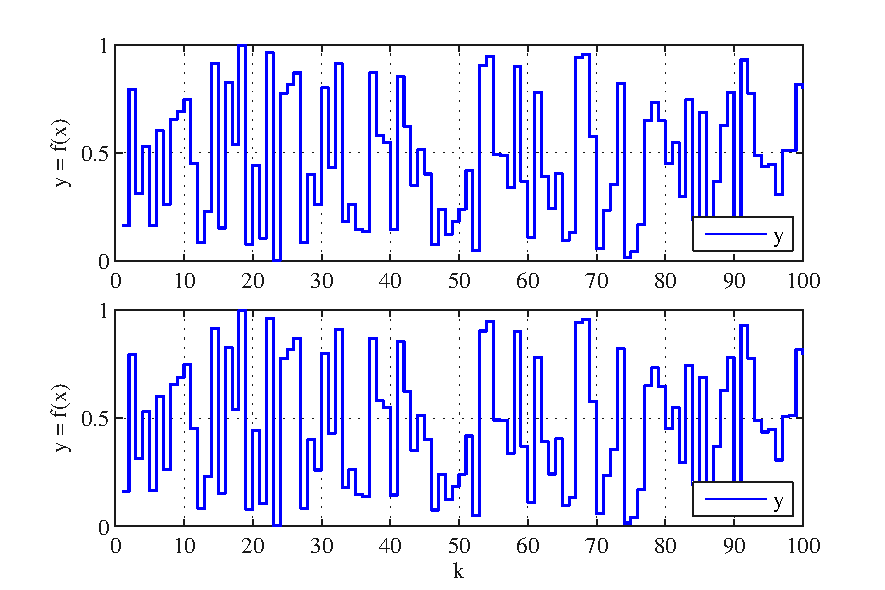
\includegraphics{images/grafik2.pdf}
	\caption{Hier steht etwas �ber die Grafik}
	\label{fig:grafik2}
\end{figure}

Hier ein Bode-Diagramm.

\begin{figure}[H]
	\centering
		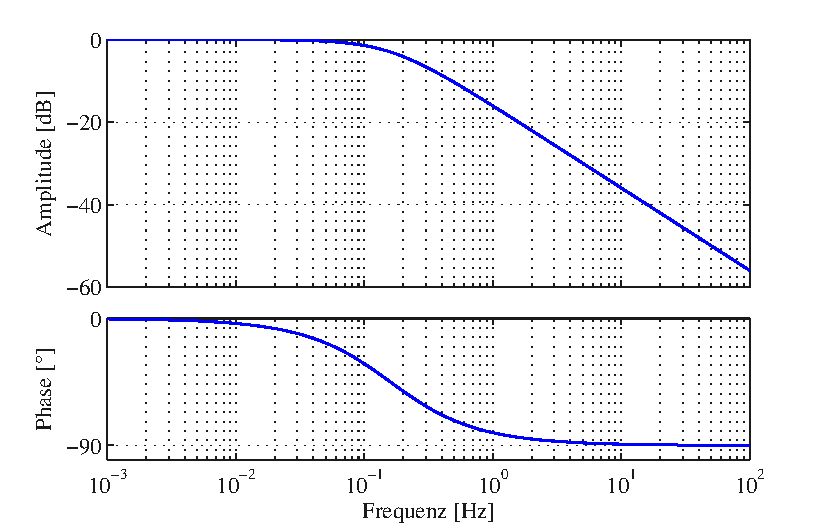
\includegraphics{images/grafik3.pdf}
	\caption{Hier steht etwas �ber die Grafik}
	\label{fig:grafik3}
\end{figure}

\subsection{Mehrere Grafiken nebeneinander}

\begin{figure}[ht]
\centering
		\subfloat[Hier k�nnen auch Formeln stehen $\m{G}(j\omega)$]{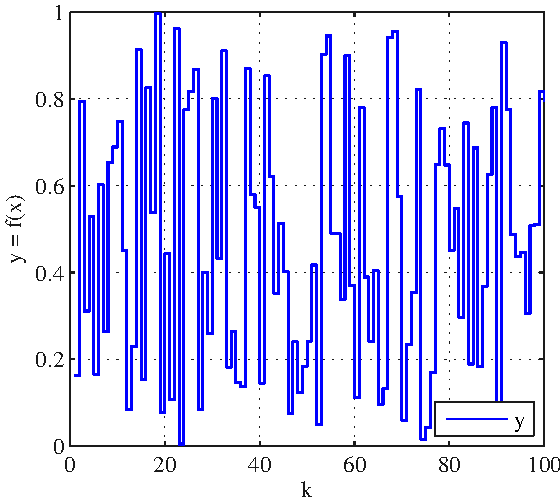
\includegraphics[width=0.50\textwidth]{images/grafik1.pdf}}
		\subfloat[Und auch hier $\m{G}(j\omega)$]{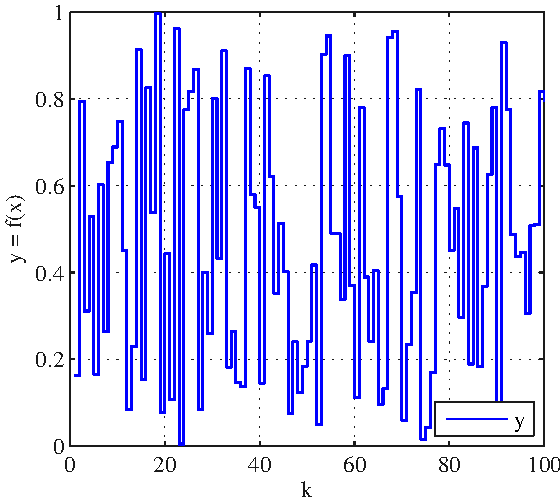
\includegraphics[width=0.50\textwidth]{images/grafik1.pdf}}
	\caption{Hier steht etwas �ber die Grafik}
	\label{fig:grafik12}
\end{figure}

\subsection{Grafik neben Text mit der Umgebung Minipage}

\begin{figure}[H]
	\begin{minipage}[b]{0.5\textwidth} 
		Dumm ist der der dummes tut. Dumm ist der der dummes tut. Dumm ist der der dummes tut. Dumm ist der der dummes tut. Dumm ist der der dummes tut. Dumm ist der der dummes tut. Dumm ist der der dummes tut. Dumm ist der der dummes tut. Dumm ist der der dummes tut.
		\vspace{4.1cm}
	\end{minipage}
	\begin{minipage}[b]{0.5\textwidth}
		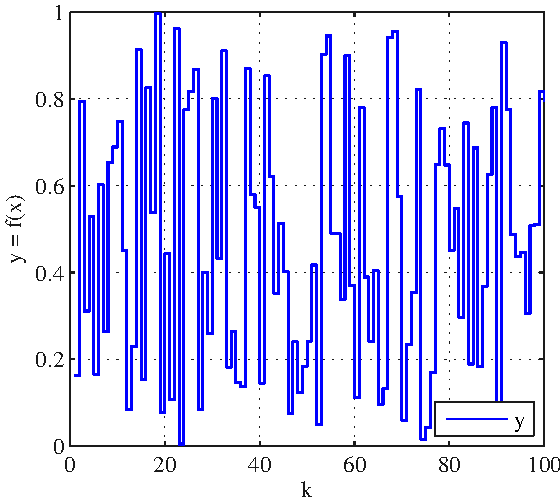
\includegraphics[width=1\textwidth]{images/grafik1.pdf}
	\end{minipage}
\end{figure}

\subsection{Eine Grafik aus Inkscape}

\begin{figure}[H]
	\centering
	\def\svgwidth{15cm}
		\input{images/skalierung_mimo_blockschaltbild.pdf_tex}
	\caption{Hier steht etwas �ber die Grafik}
	\label{fig:skalierung_mimo_blockschaltbild}
\end{figure}

%----------------------------------------------------------------------------------------------
\section{Verweise, Literaturangaben}
%----------------------------------------------------------------------------------------------

Ich bin ein Literaturverweis \cite{altb1}. Ich bin sogar zwei Literaturverweise \cite{lunze1,lunze2}.

Ich bin eine Referenz auf die Abbildung \ref{fig:skalierung_mimo_blockschaltbild}.

Ich bin eine Referenz auf das Kapitel \ref{sec:ichbineintitel}.
%------------------------------------------------------
% Importiere Anhang
%------------------------------------------------------
\appendix
\addchap{Anhang}
\refstepcounter{chapter}

%----------------------------------------------------------------------------------------------
\section{Anhang Teil 1}
%----------------------------------------------------------------------------------------------
\label{sec:anhang1}

%\begin{lstlisting}[caption=Modellparameter, label=lst:modellparameter]
\begin{lstlisting}[label=list:modellparameter]
%%%%%%%%%%%%%%%%%%%%%%%%%%%%%%%%%%%%%%%%%%%%%%%%%%%%%%%%%%%%%%%%%%%%%%%%%%%%%%%%%%%%%%%

%% Abtastzeit

P.Tsm = 1;                          % Abtastzeit der Messungen [s]
P.Ts = 0.5;                         % Abtastzeit der Regelung [s]

%% Physikalischer Normzustand DIN 1343

P.pN = 101325;                      % Normdruck [Pa]
P.TN = 273.15;                      % Normtemperatur [K]
P.Rs = 287;                         % Gaskonstante [J/kg/K]
P.rhoN = P.pN/P.Rs/P.TN;            % Normdichte [kg/m^3]
P.kappa = 1.4;                      % Isentropenexponent [-] 

%% Massenstrom und Temperatur des Kompressors

P.dmK = 0.2064;                     % Massenstrom [kg/s]
P.TK = 40 + P.TN;                   % Temperatur [K]

%% Daten der Ventilkennlinie

P.Kvs = 4;                          % Durchflusskoeffizient [m^3/h]
P.Kv0 = 0.05*P.Kvs;                 % Durchfluss bei geschlossenem Ventil
P.b = 0.5;                          % Kritischer Durchflusskoeffizient

%% Parameter des Stellmotors

P.w0 = 4;                           % Eigenkreisfrequenz [rad/s]
P.D  = 0.7;                         % D�mpfung/100 [%]
P.Tt = 2;                           % Totzeit des Aktors [s]

%% Modellparameter (Grey-Box-Systemidentifikation)

P.dmK  = 0.1803;                    % Massenstrom [kg/s]
P.TK   = 300.0001;                  % Temperatur [K]
P.Vta  = 0.1483;                    % Tankvolumen [m^3]
P.Tt   = 2.1486;                    % Totzeit [s]
P.D    = 0.8945;                    % D�mpfung/100 [%]
P.w0   = 4.2877;                    % Eigenkreisfrequenz [rad/s]
P.Kv0  = 0.3940;                    % Durchfluss bei geschlossenem Ventil
P.beta = 0.8084;                    % Zus�tzlicher Koeffizient [-]
    
%% Ventilkonstante 

P.a   = log(P.Kvs/P.Kv0);           % Ventilkonstante [-]

%%%%%%%%%%%%%%%%%%%%%%%%%%%%%%%%%%%%%%%%%%%%%%%%%%%%%%%%%%%%%%%%%%%%%%%%%%%%%%%%%%%%%%%
\end{lstlisting}

%----------------------------------------------------------------------------------------------
\section{Anhang Teil 2}
%----------------------------------------------------------------------------------------------
\label{sec:anhang2}

Dumm ist der der dummes tut. Dumm ist der der dummes tut. Dumm ist der der dummes tut. Dumm ist der der dummes tut. Dumm ist der der dummes tut. Dumm ist der der dummes tut. Dumm ist der der dummes tut. Dumm ist der der dummes tut. Dumm ist der der dummes tut.
\backmatter
%\include{zeitplan}
%------------------------------------------------------
% Erstelle Literaturverzeichnis
%------------------------------------------------------
\renewcommand{\refname}{Literaturverzeichnis}
\nocite{altb1}
\nocite{altb2}
\nocite{altb3}
\nocite{lunze1}
\nocite{lunze2}

\bibliography{references/references}{}
\bibliographystyle{alphadin}
%------------------------------------------------------
% Erstelle Abbildungsverzeichnis etc.
%------------------------------------------------------
\listoffigures
\listoftables
%------------------------------------------------------
\end{document}
%------------------------------------------------------